This appendix serves as a short introduction to the Matlab toolbox SOSTOOLS in the scope of searching for a barrier certificate for a specific closed-loop system $f_{cl}(x)$.

\section{Download and Install SOSTOOLS}
\vspace*{-3mm}
SOSTOOLS is a free third-party Matlab toolbox developed by engineering departments of four major universities. A zip file of the toolbox can be downloaded from 

\hspace{1cm} {\color{blue}{\textit{http://www.cds.caltech.edu/sostools}}}

also containing a user guide \citep{bib:sostools_manual} to sum of squares (SOS) problems and how to formulate a problem to solve it with the toolbox, along with a set of demos. 

SOSTOOLS takes as input the \gls{sos} program formulation, recasts it as a \gls{sdp} problem, calls \gls{sdp} solvers, and recasts the solution to the \gls{sdp} problem into the solution to the \gls{sos} problem. This means that the toolbox requires that an \gls{sdp} solver toolbox is installed, e.g. the SeDuMi (Self-Dual-Minimization) solver, which can be downoaded from

\hspace{1cm} {\color{blue}{\textit{http://sedumi.ie.lehigh.edu/downloads}}}

The toolboxes are activated in Matlab by adding the downloaded unzipped folders to the Matlab path.

\section{Defining an SOS Program}
\vspace*{-3mm}
As described in \citep{bib:sostools_manual}, an SOS program is initialized by declaring the independent variables as \texttt{syms} or \texttt{pvar} and optionally scalar decision variables as \texttt{syms}, and initializing an SOS program with the command \texttt{sosprogram} (in the below, grey denotes optional inputs)

\hspace*{1cm} \texttt{>> syms x1 dvar;}\\
\hspace*{1cm} \texttt{>> prog = sosprogram(x1\textcolor{grey}{,dvar});}

Now an SOS program called \texttt{prog} with the independent variable \texttt{x1} and the decision variable \texttt{dvar} has been initialized. An SOS variable \texttt{S} is added to the program by defining the monomial vector \texttt{Z} and calling the function \texttt{sossosvar}

\hspace*{1cm} \texttt{>> Z = monomials(x1,degrees);}\\
\hspace*{1cm} \texttt{>> [prog,S] = sossosvar(prog,Z);}

where \texttt{degrees} is the degrees of variables desired in the monomial; \texttt{[2 4]} would in this case give that \verb|Z = [x1^2; x1^4]| while \texttt{degrees = 0:2} would result in \verb|Z = [1; x1; x1^2]|. Declaring an SOS polynomial is done similarly to declaring an SOS variable

\hspace*{1cm} \texttt{>> Zp = monomials(x1,degrees);}\\
\hspace*{1cm} \texttt{>> [prog,P] = sospolyvar(prog,Zp);}

When all the necessary SOS variables and polynomials are defined, equalities (expression $=0$) and inequalities (expression $\geq 0$) can be defined for the program

\hspace*{1cm} \texttt{>> prog = soseq(prog,P-S);}\\
\hspace*{1cm} \texttt{>> prog = sosineq(prog,-diff(P,x1)-S);}

WHen all variables and constraints are input to the program, the solver is called with \texttt{sossolve}, which will return an overview of the precision of the solution (if any was found) as a residual error norm, number of iterations and time elapsed for solving the problem. To get the solution (coefficients) found for any of the SOS variables or polynomials, call the \texttt{sosgetsol}

\hspace*{1cm} \texttt{>> prog = sossolve(prog);}\\
\hspace*{1cm} \texttt{>> getB = sosgetsol(prog,P)}


%SeDuMi 1.3 by AdvOL, 2005-2008 and Jos F. Sturm, 1998-2003.
%Alg = 2: xz-corrector, Adaptive Step-Differentiation, theta = 0.250, beta = 0.500
%Put 5 free variables in a quadratic cone
%eqs m = 180, order n = 71, dim = 935, blocks = 8
%nnz(A) = 746 + 0, nnz(ADA) = 12522, nnz(L) = 6351
%it :     b*y       gap    delta  rate   t/tP*  t/tD*   feas cg cg  prec
%0 :            4.95E-01 0.000
%1 :   0.00E+00 1.37E-01 0.000 0.2775 0.9000 0.9000   1.00  1  0  1.4E+00
%2 :   0.00E+00 4.05E-02 0.000 0.2945 0.9000 0.9000   1.00  1  1  4.0E-01
%3 :   0.00E+00 1.11E-02 0.000 0.2736 0.9000 0.9000   1.00  1  1  1.1E-01
%4 :   0.00E+00 2.96E-03 0.000 0.2675 0.9000 0.9000   1.00  1  1  2.9E-02
%5 :   0.00E+00 9.17E-04 0.000 0.3096 0.9000 0.9000   1.00  1  1  9.1E-03
%6 :   0.00E+00 3.18E-04 0.000 0.3470 0.9107 0.9000   1.00  1  1  2.9E-03
%7 :   0.00E+00 7.91E-05 0.000 0.2486 0.8202 0.9000   1.00  1  1  7.4E-04
%8 :   0.00E+00 1.99E-05 0.000 0.2522 0.9000 0.9047   1.00  1  1  2.0E-04
%9 :   0.00E+00 6.61E-06 0.000 0.3314 0.7727 0.9000   1.00  1  2  6.7E-05
%10 :   0.00E+00 2.00E-06 0.000 0.3029 0.9000 0.9043   1.00  2  2  2.1E-05
%11 :   0.00E+00 7.15E-07 0.000 0.3573 0.8589 0.9000   1.00  1  3  7.3E-06
%12 :   0.00E+00 2.33E-07 0.000 0.3257 0.9000 0.9025   1.00  6  7  2.4E-06
%13 :   0.00E+00 8.28E-08 0.000 0.3554 0.8725 0.9000   1.00  8  9  8.5E-07
%14 :   0.00E+00 2.69E-08 0.000 0.3247 0.9000 0.9050   1.00 12 15  2.9E-07
%15 :   0.00E+00 9.41E-09 0.000 0.3499 0.9000 0.9000   1.00 19 19  9.9E-08
%16 :   0.00E+00 3.31E-09 0.000 0.3516 0.9020 0.9000   1.00 21 22  3.4E-08
%17 :   0.00E+00 1.15E-09 0.000 0.3468 0.9017 0.9000   1.00 25 24  1.1E-08
%18 :   0.00E+00 3.91E-10 0.000 0.3411 0.9007 0.9000   1.00 36 39  3.9E-09
%
%iter seconds digits       c*x               b*y
%18      0.9   Inf  0.0000000000e+00  0.0000000000e+00
%|Ax-b| =   4.6e-09, [Ay-c]_+ =   6.8E-10, |x|=  6.3e+00, |y|=  1.4e+01
%
%Detailed timing (sec)
%Pre          IPM          Post
%1.200E-02    4.640E-01    7.001E-03    
%Max-norms: ||b||=0, ||c|| = 0,
%Cholesky |add|=3, |skip| = 5, ||L.L|| = 1.03727e+08.
%
%Residual norm: 4.6491e-09
%
%iter: 18
%feasratio: 1.0000
%pinf: 0
%dinf: 0
%numerr: 0
%timing: [0.0120 0.4640 0.0070]
%wallsec: 0.4830
%cpusec: 0.9219

If no solution could be found, the degree (and thereby complexity) of some SOS variables or polynomials may be increased through their monomials, which may yield a solution to the SOS problem.


\section{Search for a Barrier Certificate with SOSTOOLS}
In the search for a barrier certificate for a given system, the above commands are used to define the polynomial $B(x)$ such that it will satisfy \autoref{eq:barrier_constraints}, restated here for convenience:
\begin{subequations}\label{eq:barrier_constraints_app}
	\begin{flalign}
		B(x) &\leq 0 \kk  \forall \hspace{2mm} x \in \mathcal{X}_0  \label{cer1_app}\\
		B(x) &> 0  \kk  \forall \hspace{2mm} x \in \mathcal{X}_u \label{cer2_app} \\
		L_{f_{cl}}B(x) &\leq 0 \kk  \forall \hspace{2mm} x \in \mathcal{X} \label{cer3_app}
	\end{flalign}
\end{subequations}

First the open-loop state space system is defined, and a controller is found according to pole placement or another preferred method. Now declare the state space variables as \verb|syms| or \verb|pvar|, initialize the SOS program with the system states and write the closed-loop system equation $f_{cl}$ with the symbolic state vector.

For the system defined, make a function $g$ that is positive in the region that will be defined as $\mathcal{X}$ i.e. has its zero level set at the desired border of the region. Make an SOS variable $q$ from a monomial vector in the state variables of appropriate degree (preferably as small as possible to keep the complexity of the problem as low as possible). Finally declare $B$ as an SOS polynomial with a monomial vector of appropriate degree and set up the SOS inequality according to Putinar's Positivstellensatz in \autoref{eq:putinar_sos}, restated here for convenience:
%\begin{subequations}\label{eq:sos_barrier_app}
\begin{align}
%h &= q_0+\sum _{j=1}^{m}q_jg_j \label{eq:putinar1_app} \\
q_0 &= h - \sum _{j=1}^{m}q_jg_j \label{eq:putinar2_app}
%\qquad \qquad \overset{\text{on } \mathbb{K}}{\Longrightarrow}\\
%0 &\leq h - \sum _{j=1}^{m}q_jg_j \label{eq:putinar3_app}
\end{align}
%\end{subequations} 	
%The SOS variables $q$ are nonnegative per definition, and as seen from \autoref{eq:putinar1_app} $h$ is positive on $\mathbb{K}$ as defined by $g$ being positive in the region $\mathbb{K}$. Outside $\mathbb{K}$ $g$ is negative, and hence the the sign of $h$ cannot be determined outside $\mathbb{K}$. Rearranging to \autoref{eq:putinar2_app}, however, the right-hand expression will always be nonnegative due to the SOS equality. 
Cf. the nonnegativity of an \gls{sos} polynomial ($q_0$), the \verb|sosineq| can be written as the right-hand side of \autoref{eq:putinar2_app}. 

In the case of defining $\mathcal{X}$ according to \autoref{cer3_app}, the polynomial $h$ can be written as $-\partial B/\partial x \, f_{cl}$.
Similar procedures are followed when defining $\mathcal{X}_0$ and $\mathcal{X}_u$: make one or more functions $g$ that is positive in the region $\mathcal{X}_0$, make SOS variable(s) $q$ of appropriate degree, and define the SOS inequality according to \autoref{eq:putinar2_app}, with $h=-B$ according to \autoref{cer1_app}; and identically make function(s) $g$ that are positive on $\mathcal{X}_u$, and define the SOS inequality \autoref{eq:putinar2_app} with $h=B$ according to \autoref{cer2_app}. The combination of \autoref{eq:barrier_constraints_app} with \autoref{eq:putinar2_app} is summarized in \autoref{eq:barrier_constraints_putinar} and restated here for convenience:
\begin{subequations}\label{eq:barrier_constraints_putinar_app}
\begin{flalign}
-B(x) &\geq 0 \kk  \forall \hspace{2mm} x \in \mathcal{X}_0 \qquad\qquad \rightarrow& 
	-B(x) - \sum _{j=1}^{m}q_jg_j &\geq 0 && \label{cer1_putinar_app}\\
B(x) &> 0 \kk  \forall \hspace{2mm} x \in \mathcal{X}_u \qquad\qquad \rightarrow& 
	B(x) - \sum _{j=1}^{m}q_jg_j &\geq 0 &&\label{cer2_putinar_app} \\
-L_{f_{cl}}B(x) &\geq 0 \kk  \forall \hspace{2mm} x \in \mathcal{X} \,\qquad\qquad \rightarrow& 
	-L_{f_{cl}}B(x) - \sum _{j=1}^{m}q_jg_j &\geq 0 && \label{cer3_putinar_app}
\end{flalign}
\end{subequations}
%Note that the inequality is on positivity in \autoref{cer2_app} whereas it is on nonnegativity in \autoref{cer2_putinar_app}. This is, however, not considered an issue in the scope of this project, as the position accuracy of the robot is not on the submillimeter level.
With all inequalities defined in the program, SOSTOOLS is now ready to solve for the barrier certificate, if any certificate exists for the given system $f_{cl}(x)$.

\subsection{Example of Barrier Certificate Search with SOSTOOLS}
This section presents an elaborate example of a state in $\mathbb{R}$ controlling a 1D first order system robot $x_1$ corresponding to the slide joint being the only degree of freedom. First the system is defined, and a controller is designed with pole placement.
\begin{lstlisting}[language=matlab]
% Define state-space system with x1 = robot position
tau = 0.11; % time constant for the robot slide
A = -1/tau;
B = 1/tau;
k = place(A,B,[-10*1/tau]);
\end{lstlisting}
Then the symbolic state variables are declared for the SOS program, and the program is initialized.
\begin{lstlisting}[language=matlab]
% Declare state variables
pvar x1

% Initialize the sum of squares program
prog = sosprogram(x1);
\end{lstlisting}
%The reference for the robot position is generated as the 1D heart position, taking into account the system gain $\bar{N}$, and the closed-loop system equation is written as a function of the sybolic state. %\textcolor{red}{Something is wrong with the reference..?}
The vector field or derivative of the state can now be defined in terms on the symbolic state variable.
\begin{lstlisting}[language=matlab]
% Vector field dx/dt = fx (closed loop)
fx = (A-B*k)*x1;
\end{lstlisting}
For ease of defining a (1D) function $g$ that is positive on an interval [$p_1\,\,\, p_2$], a parabola function is used.
\begin{lstlisting}[language=matlab]
function [a,b,c] = parabola(p1,p2)
	a = -1;
	b = a*(p1^2-p2^2)/(p2-p1);
	c = -a*p1^2-b*p1;
end
\end{lstlisting}
Now the region $\mathcal{X}$ can be defined for the slide region $\pm0.1$\,m using the Lie derivative inequality in \autoref{cer3_app}. The monomial degrees for $f$ and $B(x)$ are chosen as low as possible until a solution can be found. In this case a solution can be found for a degree of $B(x)$ that is 4.
\begin{lstlisting}[language=matlab]
% Define space X in R^n
[a,b,c] = parabola(-0.1,0.1); % get coefficients for parabola which is positive for x in [-0.1,0.1]
gX = a*x1^2+b*x1+c;
zX = monomials(vars,0:2);
[prog,qX] = sossosvar(prog,zX);
zB = monomials(x1,0:4);
[prog,Bx] = sospolyvar(prog,zB);
prog = sosineq(prog,-diff(Bx,x1)*fx-gX*qX);
\end{lstlisting}
Similarly, the region $\mathcal{X}_u$ is defined as the area between slide positions 5-10\,cm.
\begin{lstlisting}[language=matlab]
% Define space Xu in X
[a,b,c]=parabola(0.05,0.1);
gXu = a*x1^2+b*x1+c;
zXu = monomials(x1,0:2);
[prog,fXu] = sossosvar(prog,zXu);
prog = sosineq(prog,Bx-gXu*fXu);
\end{lstlisting}
And finally the region $\mathcal{X}_0$ is defined as $\mathcal{X}\setminus\mathcal{X}_u$.
\begin{lstlisting}[language=matlab]
% Define space X0 in X
[a,b,c] = parabola(-0.1,0.05);
gX0 = a*x1^2+b*x1+c;
zX0 = monomials(x1,0:2);
[prog,fX0] = sossosvar(prog,zX0);
prog = sosineq(prog,-Bx-gX0*fX0);
\end{lstlisting}
With all three areas defined according to \autoref{eq:barrier_constraints_app}, the program is ready to be solved. If a solution is found, an overview of the solution accuracy is printed in the Matlab terminal as the residual norm, number of iteration steps and solving time. To get the polynomial $B(x)$ use the function \verb|sosgetsol|.
\begin{lstlisting}[language=matlab]
% Solve for B
prog = sossolve(prog);
getB = sosgetsol(prog,Bx)
\end{lstlisting}
For this particular program, the solution barrier certificate is found to be
\begin{equation}
B(x) = 0.016168\cdot x_1^4 + 0.0064892\cdot x_1^3 + 0.00072547\cdot x_1^2 + 6.5473e\text{-}8\cdot x_1 - 2.7291e\text{-}6
\end{equation}
and is depicted in \autoref{fig:barrier_1storder_staticlim}.

\begin{figure}[htbp]
\hspace*{-12mm}
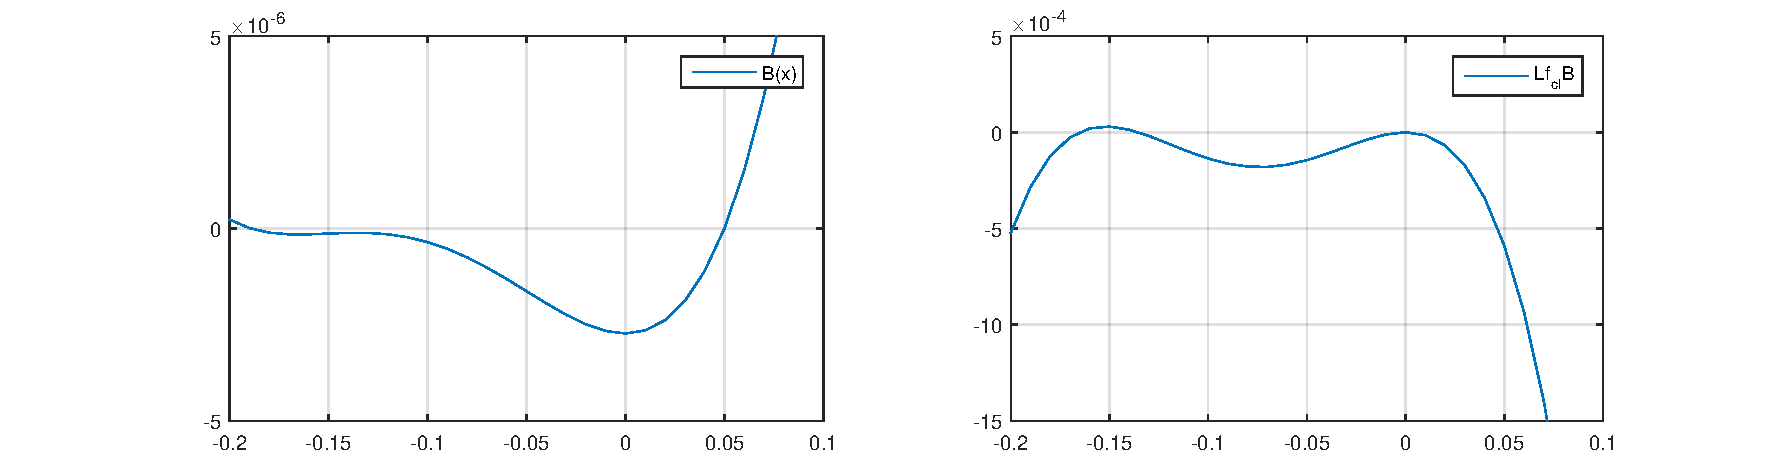
\includegraphics[width=1.1\textwidth]{1stordersys_staticlimits.pdf}
\caption{A barrier certificate is found with SOSTOOLS that complies with the requirements in \autoref{eq:barrier_constraints_app}: it is positive on $\mathcal{X}_u=\{x_1\in [0.05\,\,0.1]\}$ and negative on $\mathcal{X}_0=\{x_1\in [-0.1\,\,0.05]\}$, and its Lie derivative is nonpositive on $\mathcal{X}=\{x_1\in [-0.1\,\,0.1]\}$.}
\label{fig:barrier_1storder_staticlim}
\end{figure}

